\documentclass[utf8x]{beamer}

% This file is a solution template for:

% - Talk at a conference/colloquium.
% - Talk length is about 20min.
% - Style is ornate.

\mode<presentation>
{
  \usetheme{Warsaw}
  % or ...

  %\setbeamercovered{transparent}
  % or whatever (possibly just delete it)
}


\usepackage[english]{babel}
\usepackage{listings}
\usepackage{fancyvrb}
\usepackage{ulem}
\usepackage{color}
\usepackage{alltt}
\usepackage{hyperref}

\usepackage[utf8x]{inputenc}


\newcommand\redsout[1]{{\color{red}\sout{\hbox{\color{black}{#1}}}}}
\newcommand{\noop}{}

% or whatever

% Or whatever. Note that the encoding and the font should match. If T1
% does not look nice, try deleting the line with the fontenc.


\title{Meta-Tracing in the PyPy Project}

\author[Carl Friedrich Bolz et. al.]{\emph{Carl Friedrich Bolz}\inst{1} \and Antonio Cuni\inst{1} \and Maciej Fijałkowski\inst{2} \and Michael Leuschel\inst{1} \and Samuele Pedroni\inst{3} \and Armin Rigo\inst{1} \and many~more}
% - Give the names in the same order as the appear in the paper.
% - Use the \inst{?} command only if the authors have different
%   affiliation.

\institute[Heinrich-Heine-Universität Düsseldorf]
{$^1$Heinrich-Heine-Universität Düsseldorf, STUPS Group, Germany \and

 $^2$merlinux GmbH, Hildesheim, Germany \and

 $^3$Canonical
}

\date{Foundations of Scription Languages, Dagstuhl, 5th January 2012}
% - Either use conference name or its abbreviation.
% - Not really informative to the audience, more for people (including
%   yourself) who are reading the slides online


% If you have a file called "university-logo-filename.xxx", where xxx
% is a graphic format that can be processed by latex or pdflatex,
% resp., then you can add a logo as follows:




% Delete this, if you do not want the table of contents to pop up at
% the beginning of each subsection:
%\AtBeginSubsection[]
%{
%  \begin{frame}<beamer>
%    \frametitle{Outline}
%    \tableofcontents[currentsection,currentsubsection]
%  \end{frame}
%}


% If you wish to uncover everything in a step-wise fashion, uncomment
% the following command: 

%\beamerdefaultoverlayspecification{<+->}


\begin{document}

\begin{frame}
  \titlepage
\end{frame}

\begin{frame}
  \frametitle{Good JIT Compilers for Scripting Languages are Hard}
  \begin{itemize}
      \item recent languages like Python, Ruby, JS, PHP have complex core semantics
      \item many corner cases, even hard to interpret correctly
      \item particularly in contexts where you have limited resources (like
      academic, Open Source)
  \end{itemize}
  \pause
  \begin{block}{Problems}
      \begin{enumerate}
          \item implement all corner-cases of semantics correctly
          \item ... and the common cases efficiently
          \item while maintaing reasonable simplicity in the implementation
      \end{enumerate}
  \end{block}
\end{frame}

\begin{frame}
  \frametitle{Example: Attribute Reads in Python}
  What happens when an attribute \texttt{x.m} is read? (simplified)
  \pause
  \begin{itemize}
      \item check for \texttt{x.\_\_getattribute\_\_}, if there, call it
      \pause
      \item look for the attribute in the object's dictionary, if it's there, return it
      \pause
      \item walk up the MRO and look in each class' dictionary for the attribute
      \pause
      \item if the attribute is found, call its \texttt{\_\_get\_\_} attribute and return the result
      \pause
      \item if the attribute is not found, look for \texttt{x.\_\_getattr\_\_}, if there, call it
      \pause
      \item raise an \texttt{AttributeError}
  \end{itemize}
\end{frame}

\begin{frame}
  \frametitle{An Interpreter}
  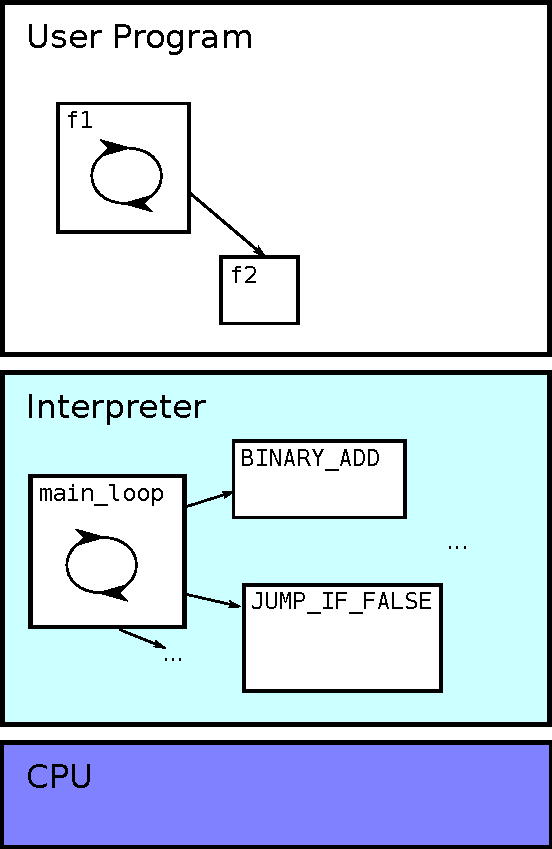
\includegraphics[scale=0.5]{figures/trace01.pdf}
\end{frame}

\begin{frame}
  \frametitle{A Tracing JIT}
  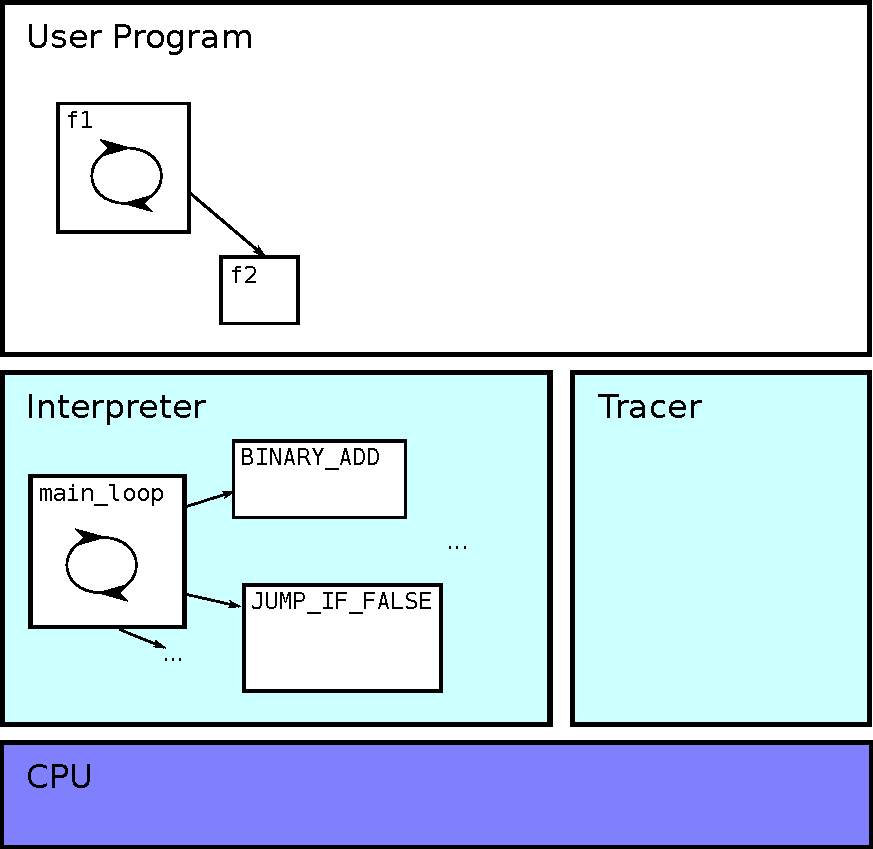
\includegraphics[scale=0.5]{figures/trace02.pdf}
\end{frame}

\begin{frame}
  \frametitle{A Tracing JIT}
  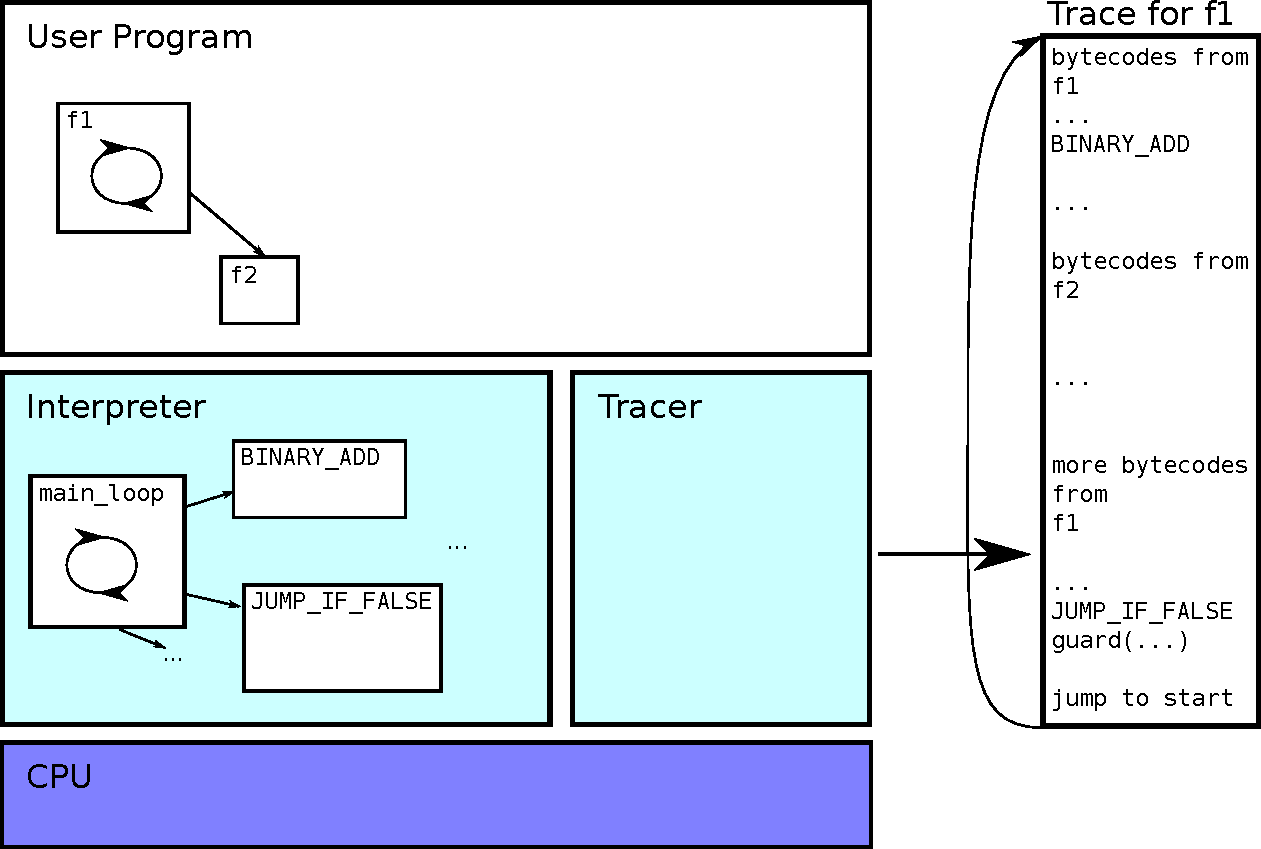
\includegraphics[scale=0.5]{figures/trace03.pdf}
\end{frame}

\begin{frame}
  \frametitle{A Tracing JIT}
  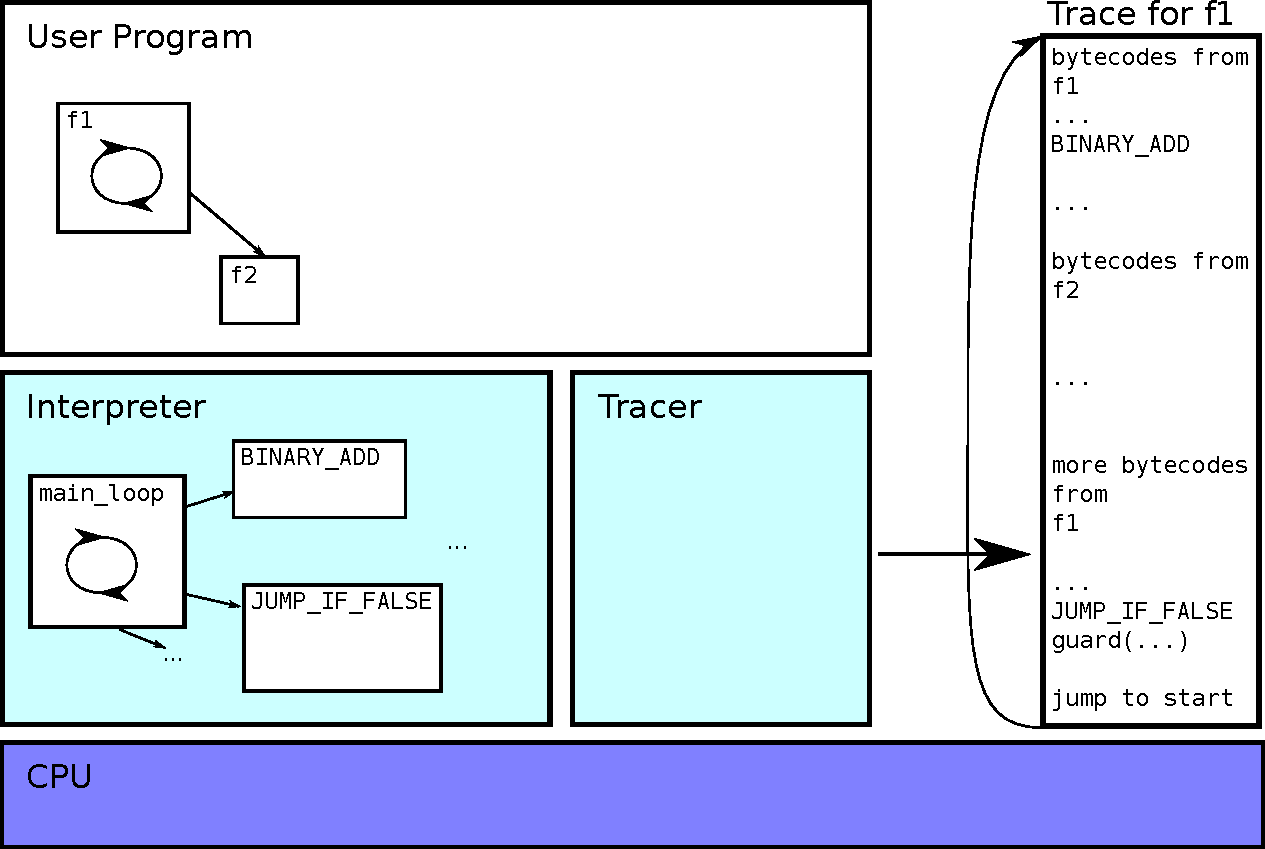
\includegraphics[scale=0.5]{figures/trace04.pdf}
\end{frame}

\begin{frame}
  \frametitle{Tracing JITs}
  Advantages:
  \begin{itemize}
      \item can be added to existing VM
      \item interpreter does a lot of work
      \item can fall back to interpreter for uncommon paths
  \end{itemize}
  \pause
  \begin{block}{Problems}
      \begin{itemize}
          \item traces typically contain bytecodes
          \item many scripting languages have bytecodes that contain complex logic
          \item need to expand the bytecode in the trace into something more explicit
          \item this duplicates the language semantics in the tracer/optimizer
      \end{itemize}
  \end{block}
\end{frame}

\begin{frame}
  \frametitle{Idea of Meta-Tracing}
  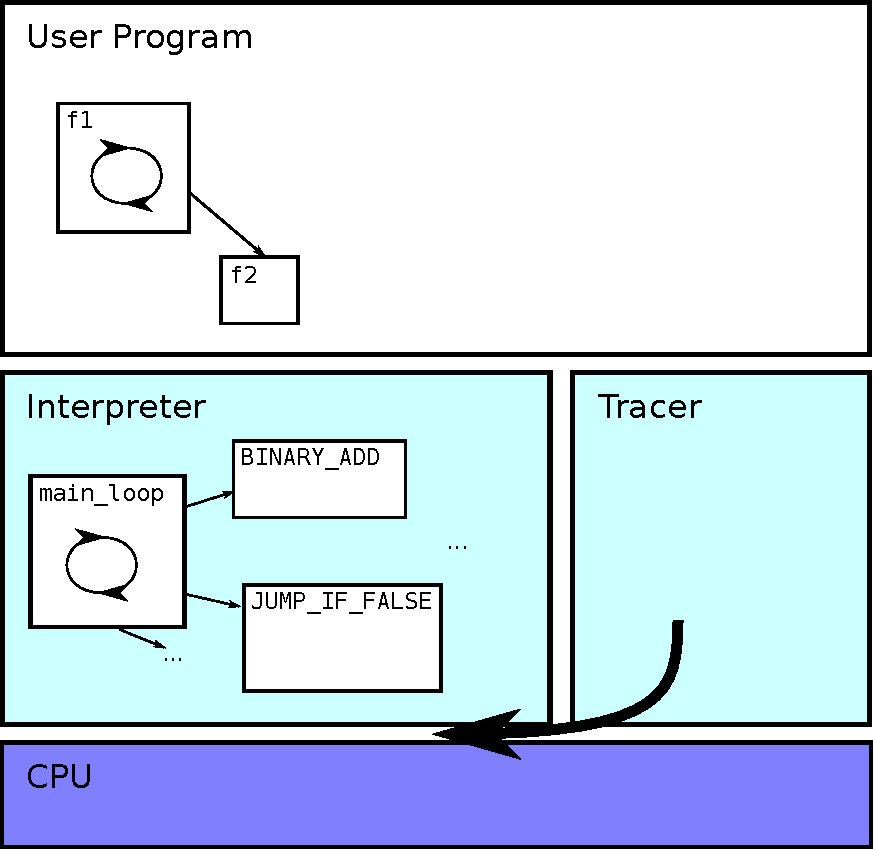
\includegraphics[scale=0.5]{figures/trace05.pdf}
\end{frame}

\begin{frame}
  \frametitle{Meta-Tracing}
  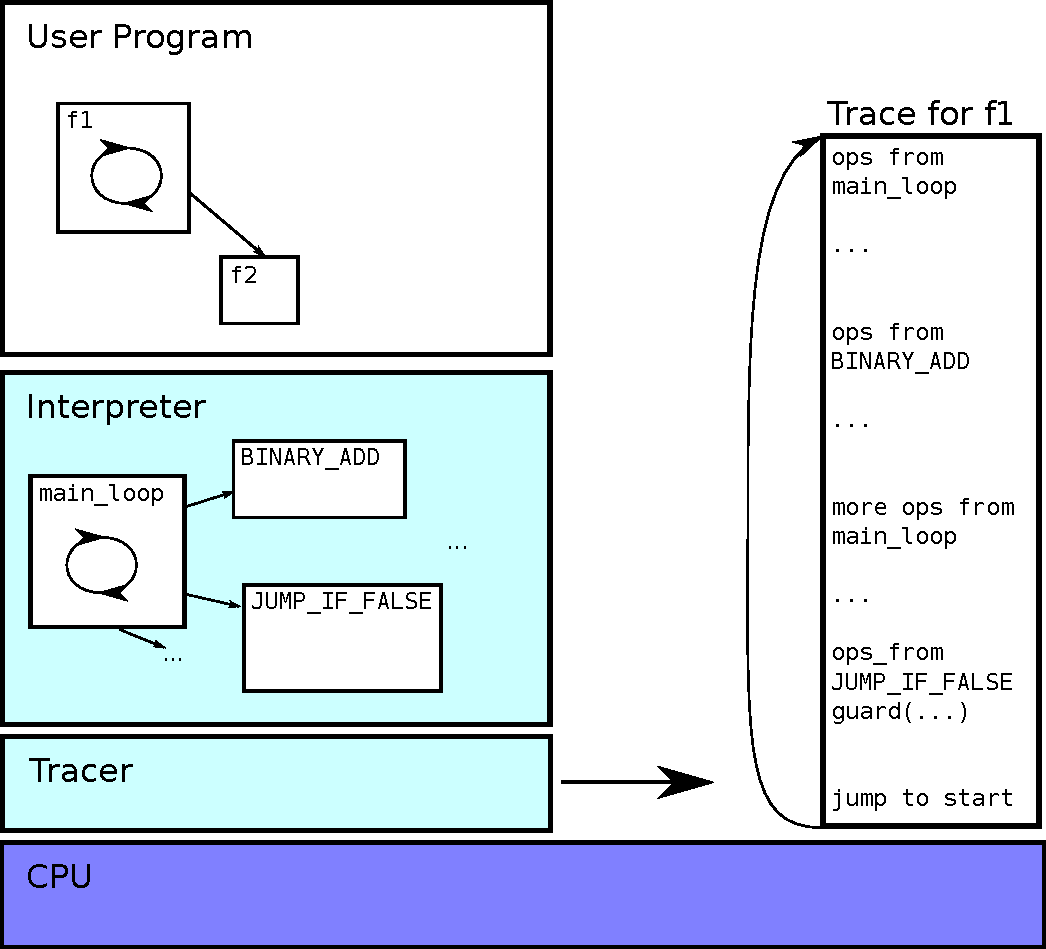
\includegraphics[scale=0.5]{figures/metatrace01.pdf}
\end{frame}

\begin{frame}
  \frametitle{Meta-Tracing JITs}
  \begin{block}{Advantages:}
    \begin{itemize}
        \item semantics are always like that of the interpreter
        \item trace fully contains language semantics
        \item meta-tracers can be reused for various interpreters
    \end{itemize}
  \end{block}
  \pause
  a few meta-tracing systems have been built:
  \begin{itemize}
      \item Sullivan et.al. describe a meta-tracer using the Dynamo RIO system
      \item Yermolovich et.al. run a Lua implementation on top of a tracing JS implementation
      \item SPUR is a tracing JIT for CLR bytecodes, which is used to speed up a JS implementation in C\#
  \end{itemize}
\end{frame}

\begin{frame}
  \frametitle{PyPy}
  A general environment for implementing scripting languages
  \pause
  \begin{block}{Approach}
      \begin{itemize}
          \item write an interpreter for the language in RPython
          \item compilable to an efficient C-based VM
          \pause
          \item (RPython is a restricted subset of Python)
      \end{itemize}
  \end{block}
  \pause
\end{frame}

\begin{frame}
  \frametitle{PyPy's Meta-Tracing JIT}
  \begin{itemize}
      \item PyPy contains a meta-tracing JIT for interpreters in RPython
      \item needs a few source-code hints (or annotations) \emph{in the interpreter}
      \item allows interpreter-author to express language specific type feedback
      \item contains powerful general optimizations
      \pause
      \item general techniques to deal with reified frames
  \end{itemize}
\end{frame}



\begin{frame}
  \frametitle{Language Implementations Done with PyPy}
  \begin{itemize}
      \item Most complete language implemented: Python
      \item regular expression matcher of Python standard library
      \item A reasonably complete Prolog
      \item Converge (previous talk)
      \item lots of experiments (Squeak, Gameboy emulator, JS, start of a PHP, Haskell, ...)
  \end{itemize}
\end{frame}


\begin{frame}
  \frametitle{Some Benchmarks for Python}
  \begin{itemize}
      \item benchmarks done using PyPy's Python interpreter
      \item about 30'000 lines of code
  \end{itemize}
\end{frame}

\begin{frame}
  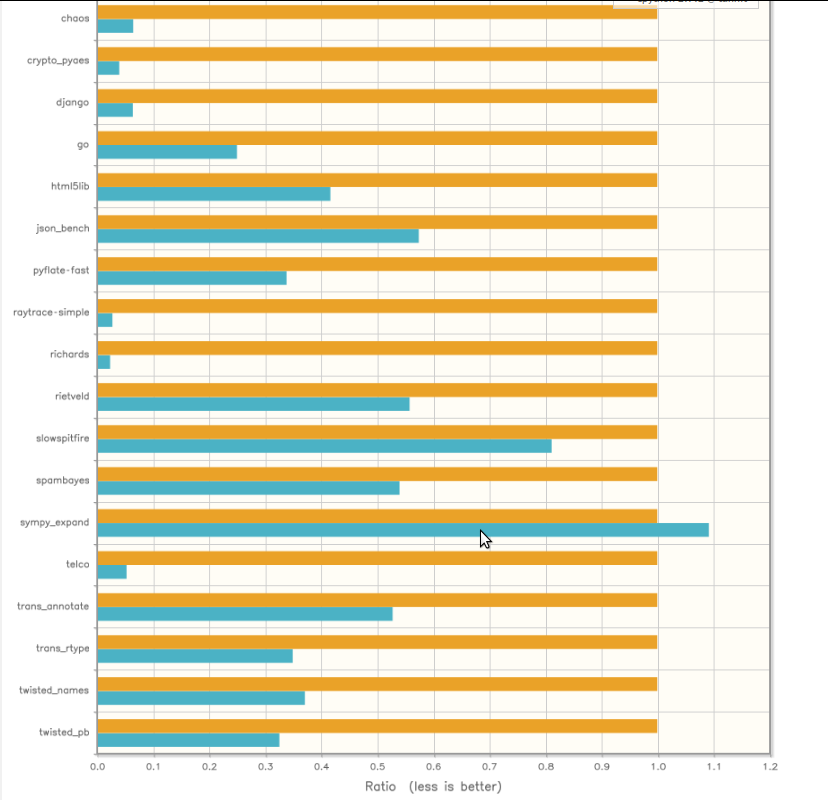
\includegraphics[scale=0.3]{figures/all_numbers.png}
\end{frame}

\begin{frame}
  \frametitle{Telco Benchmark}
  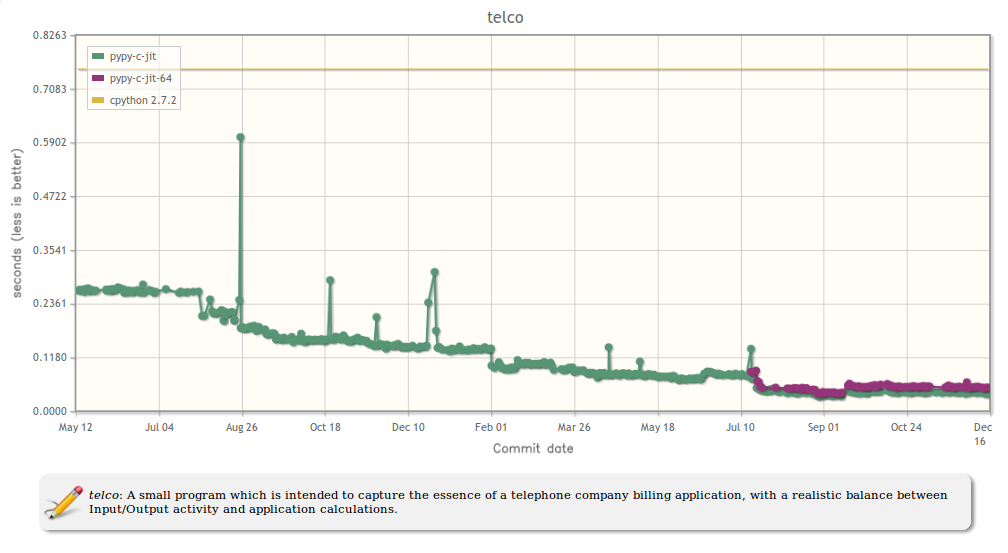
\includegraphics[scale=0.3]{figures/telco.png}
\end{frame}

\begin{frame}
  \frametitle{Conclusion}
  \begin{itemize}
      \item writing good JITs for recent scripting languages is too hard!
      \item only reasonable if the language is exceptionally simple
      \item or if somebody has a lot of money
      \item PyPy is one point in a large design space of meta-solutions
      \item uses tracing on the level of the interpreter (meta-tracing) to get speed
      \pause
      \item \textbf{In a way, the exact approach is not too important: let's write more meta-tools!}
  \end{itemize}
\end{frame}

\begin{frame}
  \frametitle{Thank you! Questions?}
  \begin{itemize}
      \item writing good JITs for recent scripting languages is too hard!
      \item only reasonable if the language is exceptionally simple
      \item or if somebody has a lot of money
      \item PyPy is one point in a large design space of meta-solutions
      \item uses tracing on the level of the interpreter (meta-tracing) to get speed
      \item \textbf{In a way, the exact approach is not too important: let's write more meta-tools!}
  \end{itemize}
\end{frame}

\begin{frame}
  \frametitle{Possible Further Slides}
  \hyperlink{necessary-hints}{\beamergotobutton{}} Getting Meta-Tracing to Work

  \hyperlink{feedback}{\beamergotobutton{}} Language-Specific Runtime Feedback

  \hyperlink{optimizations}{\beamergotobutton{}} Powerful General Optimizations

  \hyperlink{virtualizables}{\beamergotobutton{}} Optimizing Reified Frames

  \hyperlink{which-langs}{\beamergotobutton{}} Which Languages Can Meta-Tracing be Used With?

  \hyperlink{OOVM}{\beamergotobutton{}} Using OO VMs as an implementation substrate

  \hyperlink{PE}{\beamergotobutton{}} Comparison with Partial Evaluation

\end{frame}

\begin{frame}[label=necessary-hints]
  \frametitle{Getting Meta-Tracing to Work}
  \begin{itemize}
      \item Interpreter author needs add some hints to the interpreter
      \item one hint to identify the bytecode dispatch loop
      \item one hint to identify the jump bytecode
      \item with these in place, meta-tracing works
      \item but produces non-optimal code
  \end{itemize}
\end{frame}


\begin{frame}[label=feedback]
  \frametitle{Language-Specific Runtime Feedback}
  Problems of Naive Meta-Tracing:
  \begin{itemize}
      \item user-level types are normal instances on the implementation level
      \item thus no runtime feedback of user-level types
      \item tracer does not know about invariants in the interpreter
  \end{itemize}
  \pause
  \begin{block}{Solution in PyPy}
      \begin{itemize}
          \item introduce more hints that the interpreter-author can use
          \item hints are annotation in the interpreter
          \item they give information to the meta-tracer
          \pause
          \item one to induce runtime feedback of arbitrary information (typically types)
          \item the second one to influence constant folding
      \end{itemize}
  \end{block}
\end{frame}


\begin{frame}[label=optimizations]
  \frametitle{Powerful General Optimizations}
  \begin{itemize}
      \item Very powerful general optimizations on traces
      \pause
      \begin{block}{Heap Optimizations}
        \begin{itemize}
            \item escape analysis/allocation removal
            \item remove short-lived objects
            \item gets rid of the overhead of boxing primitive types
            \item also reduces overhead of constant heap accesses
        \end{itemize}
      \end{block}
  \end{itemize}
\end{frame}

\begin{frame}[label=virtualizables]
  \frametitle{Optimizing Reified Frames}
  \begin{itemize}
      \item Common problem in scripting languages
      \item frames are reified in the language, i.e. can be accessed via reflection
      \item used to implement the debugger in the language itself
      \item or for more advanced usecases (backtracking in Smalltalk)
      \item when using a JIT, quite expensive to keep them up-to-date
      \pause
      \begin{block}{Solution in PyPy}
          \begin{itemize}
              \item General mechanism for updating reified frames lazily
              \item use deoptimization when frame objects are accessed by the program
              \item interpreter just needs to mark the frame class
          \end{itemize}
      \end{block}
  \end{itemize}
\end{frame}


\begin{frame}[label=which-langs]
  \frametitle{Bonus: Which Languages Can Meta-Tracing be Used With?}
  \begin{itemize}
      \item To make meta-tracing useful, there needs to be some kind of runtime variability
      \item that means it definitely works for all dynamically typed languages
      \item ... but also for other languages with polymorphism that is not resolvable at compile time
      \item most languages that have any kind of runtime work
  \end{itemize}
\end{frame}

\begin{frame}[label=OOVM]
  \frametitle{Bonus: Using OO VMs as an implementation substrate}
  \begin{block}{Benefits}
      \begin{itemize}
          \item higher level of implementation
          \item the VM supplies a GC and mostly a JIT
          \item better interoperability than what the C level provides
          \item \texttt{invokedynamic} should make it possible to get language-specific runtime feedback
      \end{itemize}
  \end{block}
  \pause
  \begin{block}{Problems}
      \begin{itemize}
          \item can be hard to map concepts of the scripting language to
            the host OO VM
          \item performance is often not improved, and can be very bad, because of this
            semantic mismatch
          \item getting good performance needs a huge amount of tweaking
          \item tools not really prepared to deal with people that care about
          the shape of the generated assembler
      \end{itemize}
  \end{block}
  \pause
\end{frame}

\begin{frame}[label=PE]
  \frametitle{Bonus: Comparison with Partial Evaluation}
  \begin{itemize}
      \pause
      \item the only difference between meta-tracing and partial evaluation is that meta-tracing works
      \pause
      \item ... mostly kidding
      \pause
      \item very similar from the motivation and ideas
      \item PE was never scaled up to perform well on large interpreters
      \item classical PE mostly ahead of time
      \item PE tried very carefully to select the right paths to inline and optimize
      \item quite often this fails and inlines too much or too little
      \item tracing is much more pragmatic: simply look what happens
  \end{itemize}
\end{frame}

\end{document}
